Para los tres modelos planteados en el trabajo práctico estimaremos el error cuadrático medio utilizando el método de resampleo: Leave One Out Cross Validation, obtuvimos los siguientes resultados.

\begin{center}
    \begin{tabular}{|c|c|}
        \hline
        Modelo & $\hat{ECM}$ \\ \hline
        M1 & $21.39$ \\ \hline
        M2 & $14.34$ \\ \hline
        M3 & $15.05$ \\ \hline
    \end{tabular}
\end{center}
De la tabla podemos ver que el modelo que mejor error cuadrático medio obtiene es el modelo 2.
\begin{figure}[H]
    \centering
    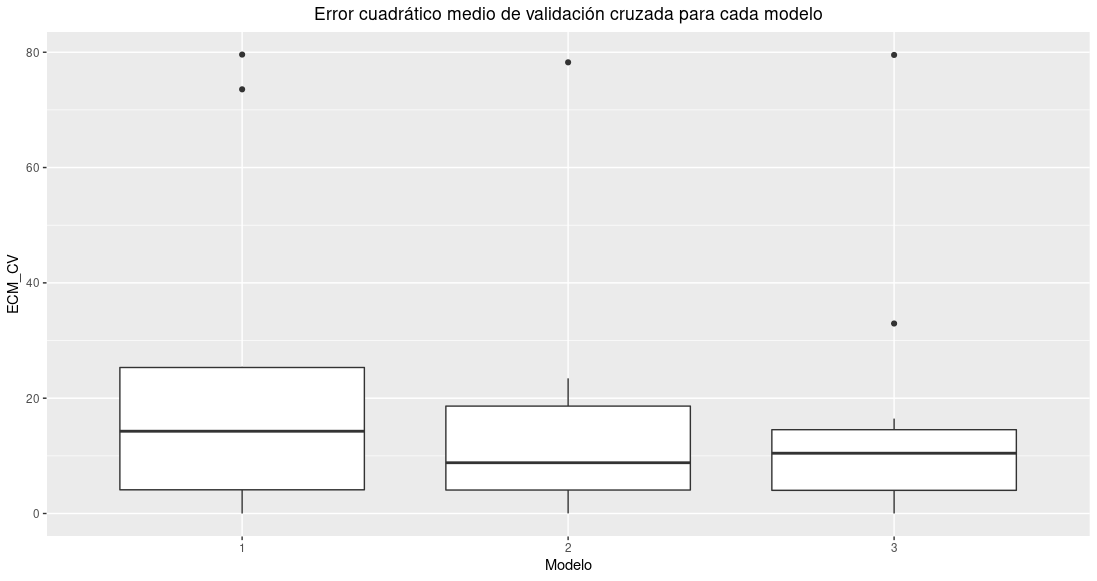
\includegraphics[width=0.8\textwidth]{resources/boxplots_modelos.png}
\end{figure}

En este gráfico en el cual los modelos están ordenados descendentemente por complejidad, podemos ver sobre el rango intercuartílico como que a medida que la complejidad disminuye lo hace la dispersión. Reconocemos particularmente ambos valores atípicos identificados en el ítem 1, los cuales generan un aumento fuerte en la media de la estimación del error cuadrático medio.
\vskip0.2cm
Siendo que en el ejercicio 5 en los modelos con 2 y 3 variables observamos valores para $R^2_{adj}$ y $CP$ muy parecidos a lo ideal, queremos ver cómo se comportarán estimando el error cuadrático medio con LOOCV:
\begin{equation}\tag{M4}
    Y = 51.14 + 1.71 \cdot X_2 + 0.73 \cdot X_3
\end{equation}

\begin{equation}\tag{M5}
    Y = 55.88 - 0.26 \cdot X_1 + 1.47 \cdot X_2 + 0.73 \cdot X_3
\end{equation}

Para estos obtuvimos los siguientes resultados:

\begin{center}
    \begin{tabular}{|c|c|}
        \hline
        Modelo & $\hat{ECM}$ \\ \hline
        M4 & $8.12$ \\ \hline
        M5 & $11.85$ \\ \hline
    \end{tabular}
\end{center}

Podemos ver que para el modelo M4, aquel que se compone sólo por las covariables $X_2$ y $X_3$ obtuvo el menor ECM de LOOCV. Queremos remarcar de esta regresión lineal que, además de tener un alto $CP$ y un alto $R^2_{adj}$, se corresponde con lo observado en el ítem 1 para los índices de correlación de Pearson. \\Esto es:
entre $X_2$ y $X_3$ el índice de correlación es lo suficientemente bajo como para permitirnos decir que no tienen una relación lineal entre sí. Sin embargo, ambos coeficientes $X_2$ e $Y$ y $X_3$ e $Y$ son de modulo cercano a $1$, por lo que: esto nos indica que las variables $X_2$ y $X_3$ permiten estimar a $Y$ con coeficientes muy significativos y casi sin relación lineal entre sí, y esto teóricamente debería resultar en una buena regresión.
 


